%% ARC_GRI30_NOx22 paper, preprint v1, 2026-11-17 (Spain time). Target: Combustion and Flame (elsarticle).
%% Source: the merged Claude Doc draft https://claude.ai/artifact/M5mtw4X5dG4RM9AiemtYWX and results/sim1/ARC22.
%% \todo{} = must be resolved before submission. refs.bib entries are from memory: check each one.
%% Build: pdflatex arc22_cnf && bibtex arc22_cnf && pdflatex arc22_cnf && pdflatex arc22_cnf
\documentclass[preprint,review,12pt]{elsarticle}

\usepackage[T1]{fontenc}
\usepackage{lmodern}
\usepackage{amsmath,amssymb}
\usepackage{graphicx}
\usepackage{booktabs}
\usepackage{lineno}
\usepackage{xcolor}
\usepackage{tikz}
\usetikzlibrary{positioning,arrows.meta}
\usepackage[hidelinks]{hyperref}
\providecommand{\todo}[1]{}
\renewcommand{\todo}[1]{\textcolor{red}{[TODO: #1]}}
\newcommand{\ce}[1]{\ensuremath{\mathrm{#1}}}
\linenumbers
\journal{Combustion and Flame}

\begin{document}
\sloppy
\begin{frontmatter}

\title{ARC\_GRI30\_NOx22: an analytically reduced GRI-Mech~3.0 with NO$_x$, validated in a radiating burner flame}

\author[a]{Javier \todo{surname}}
\author[a]{\todo{co-authors}}
\address[a]{\todo{affiliation}}

\begin{abstract}
We present ARC\_GRI30\_NOx22, an analytically reduced chemistry (ARC) for methane--air combustion with nitrogen
oxides, derived from GRI-Mech~3.0 (53 species, 325 reactions). Two-pass DRGEP with second-generation path-flux
analysis gives a 43-species, 262-reaction skeletal set; a CSP slow-subspace analysis then splits it into 22
transported species and 21 quasi-steady radicals. The radicals follow from a linearized QSSA in which 11
radical--radical directions are dropped from the balances, and an element projection onto \ce{CO_{2}}, \ce{H_{2}O},
\ce{O_{2}} and \ce{N_{2}} restores C/H/O/N conservation. The largest Jacobian eigenvalue falls 140-fold. Two independent
checks against GRI-Mech~3.0 agree: the original reduction reproduces ignition delays within 0.93\,\% (49 cases,
1--10\,atm), laminar flame speeds within 1.3\,\% at 1\,atm and 4.7\,\% at 5\,atm, and PSR NO within 3\,\% down to
near blow-out; an independent rebuild gives the same net production rates (maximum relative difference $2\times10^{-8}$), ignition delays within
1.43\,\% up to $\phi=2$ and 1\,atm flame speeds within 1.3\,\%, and locates the weak point in hot rich gas. As an
OpenFOAM chemistry library, the ARC was used for direct integration of a laminar, radiating, axisymmetric \ce{CH_{4}}
jet flame under a pot. In the same code as full GRI-Mech~3.0 it reproduces the flame to 3.2\,K in mean hot-cell
temperature, with OH, CO and NO within 7\,\% (relative L1: volume-weighted mean absolute difference over the mean of the larger value), and ignites it at the same time, at 2.7--3.4 times lower
cost per step; HCN and \ce{N_{2}O} are the weakest species (17--23\,\%). The 38.6\,K difference to a Fluent GRI-Mech~3.0
solution on the same mesh is below the 48.8\,K that separates the two codes with identical chemistry.
\end{abstract}

\begin{keyword}
analytically reduced chemistry \sep quasi-steady-state approximation \sep NO$_x$ \sep GRI-Mech 3.0 \sep
direct integration \sep laminar diffusion flame
\end{keyword}
\end{frontmatter}

%% ---------------------------------------------------------------------------------------------------------------
\section{Introduction}

Direct integration of detailed \ce{CH_{4}}/air chemistry is the accuracy reference for reacting CFD, but it is
costly. Its cost scales with the number of transported species and with the stiffness of the radical subsystem:
GRI-Mech~3.0~\cite{gri30} has Jacobian eigenvalues near $5\times10^{8}$\,s$^{-1}$, from short-lived radicals such as
NNH, CH, C, \ce{CH_{2}(S)}, \ce{H_{2}CN} and CN, so implicit integrators pay $O(N^3)$ linear algebra per cell and step.
Smaller mechanisms such as GA18~\cite{ga18} (18 species, 92 reactions), used so far in this project, are cheaper but carry no
nitrogen chemistry, so they cannot predict NO.

Analytically reduced chemistry keeps the elementary reactions of the detailed mechanism and removes only the fast
radicals from the transported set, solving their quasi-steady balances algebraically at every rate
evaluation~\cite{lu2009review,felden2018}. Pathways stay explicit, at a cost close to a skeletal mechanism. This work:
\begin{enumerate}
\item Documents the reduction of GRI-Mech~3.0 to 22 transported species that keep all six NO$_x$ pathways
(thermal, prompt, \ce{N_{2}O}-intermediate, NNH, HCCO/HCNO reburning and NO/\ce{NO_{2}} conversion), with at least a
100-fold stiffness reduction;
\item Validates it against GRI-Mech~3.0 in homogeneous reactors and 1D premixed flames, twice: with the original
reduction and with an independent rebuild of it;
\item Validates it in a multidimensional, radiating laminar diffusion flame against direct integration with full
GRI-Mech~3.0, in the same CFD code and against a second code.
\end{enumerate}
The available GRI-Mech~3.0 reference was computed in Fluent~\cite{fluent}, while the ARC runs in
OpenFOAM~\cite{openfoam}. We therefore also run full GRI-Mech~3.0 in OpenFOAM, which isolates the mechanism error,
and measure the OpenFOAM--Fluent difference with identical GA18 chemistry, which bounds what a cross-code comparison
can show.

%% ---------------------------------------------------------------------------------------------------------------
\section{Reduction procedure}
\label{sec:reduction}

The reduction runs in five stages, each checked against GRI-Mech~3.0 before the next (Fig.~\ref{fig:pipeline}).
Numbers marked (report) are taken from the technical report of the original reduction~\cite{arcreport}, which
documents the generation scripts and their acceptance tests. Numbers marked (checked) were recomputed for this paper,
independently of those scripts, from \texttt{gri30.yaml} with Cantera~3.2~\cite{cantera} and a rebuilt
implementation of the mechanism (Section~\ref{sec:rebuild}).

\begin{figure}[t]
\centering
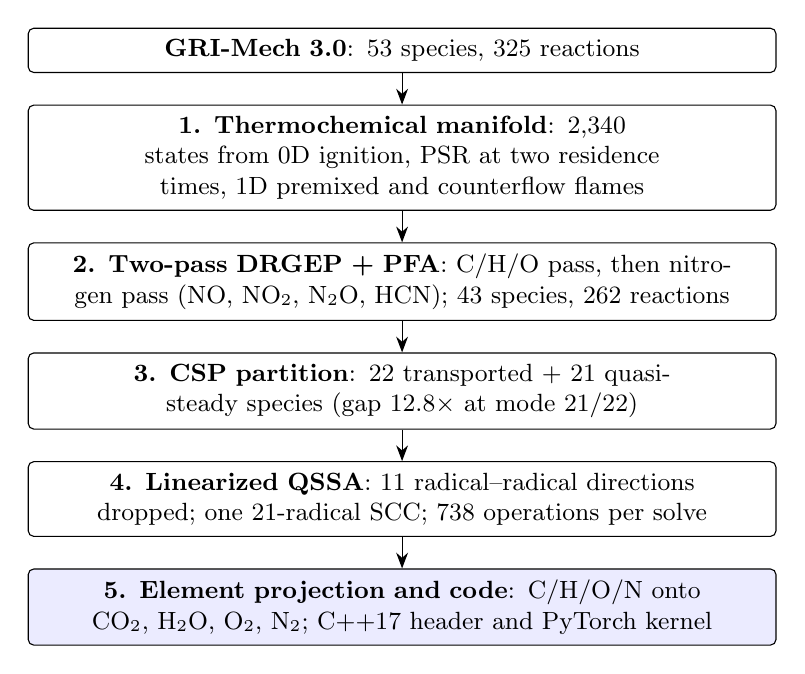
\begin{tikzpicture}[node distance=4mm, every node/.style={font=\small},
  box/.style={draw, rounded corners=2pt, align=center, text width=0.76\linewidth, inner sep=4pt},
  arr/.style={-{Stealth[length=2mm]}}]
\node[box] (g) {\textbf{GRI-Mech 3.0}: 53 species, 325 reactions};
\node[box, below=of g] (m) {\textbf{1. Thermochemical manifold}: 2,340 states from 0D ignition, PSR at two residence times,
1D premixed and counterflow flames};
\node[box, below=of m] (s) {\textbf{2. Two-pass DRGEP + PFA}: C/H/O pass, then nitrogen pass (NO, \ce{NO_{2}}, \ce{N_{2}O},
HCN); 43 species, 262 reactions};
\node[box, below=of s] (c) {\textbf{3. CSP partition}: 22 transported + 21 quasi-steady species (gap $12.8\times$ at
mode 21/22)};
\node[box, below=of c] (q) {\textbf{4. Linearized QSSA}: 11 radical--radical directions dropped; one 21-radical
SCC; 738 operations per solve};
\node[box, below=of q, fill=blue!8] (p) {\textbf{5. Element projection and code}: C/H/O/N onto \ce{CO_{2}}, \ce{H_{2}O},
\ce{O_{2}}, \ce{N_{2}}; C++17 header and PyTorch kernel};
\foreach \a/\b in {g/m, m/s, s/c, c/q, q/p} \draw[arr] (\a) -- (\b);
\end{tikzpicture}
\caption{The reduction chain from GRI-Mech~3.0 to ARC\_GRI30\_NOx22. Each stage was checked against GRI-Mech~3.0
before the next.}
\label{fig:pipeline}
\end{figure}

\subsection{Thermochemical manifold}
The reduction targets are evaluated on 2,340 states sampled with Cantera (report): 45 constant-pressure ignition
trajectories ($p=1,5,10$\,atm, $T_0=1150,1350,1550$\,K, $\phi=0.6$--1.5, each with a 3\,ms post-ignition hold);
54 perfectly stirred reactor states at $\tau=3$\,ms (thermal NO) and $1.15\,\tau_{\rm bo}$ (prompt, \ce{N_{2}O} and NNH
NO); 6 freely propagating premixed flames ($p=1,5$\,atm, $\phi=0.7,1.0,1.3$, $T_u=300$\,K); and 2 counterflow
\ce{CH_{4}}/air diffusion flamelets at 1\,atm.

\subsection{Skeletal reduction: two-pass DRGEP and PFA}
For species $A$ in reaction $r$, with net stoichiometric coefficient $\nu_{A,r}$ and net rate of progress $\omega_r$
(kmol\,m$^{-3}$\,s$^{-1}$), the production rate $P_A$ and consumption rate $C_A$ of $A$ sum the positive and negative
contributions of all reactions, and the direct interaction coefficient $r_{AB}$ measures the fraction of the larger of
the two that passes through reactions involving species $B$ ($\delta_{B,r}=1$ if $B$ is a reactant, product or
explicit third body of reaction $r$, 0 otherwise):
\begin{gather}
P_A=\sum_r \max(\nu_{A,r}\omega_r,0),\qquad C_A=\sum_r \max(-\nu_{A,r}\omega_r,0),\label{eq:pc}\\
r_{AB}=\frac{\left|\sum_r \nu_{A,r}\,\omega_r\,\delta_{B,r}\right|}{\max(P_A,C_A)},
\end{gather}
Here $B$ is any other species of the mechanism. The DRGEP importance~\cite{pepiot2008drgep} of $B$ is the
strongest product of interaction coefficients along any path $\mathcal{P}$ of species from a target $T$ to $B$, over
the set $\mathcal{T}$ of target species; a species whose largest importance over all manifold states stays below the
threshold is removed:
\begin{equation}
R_{\mathcal{T}\to B}=\max_{T\in\mathcal{T}}\ \max_{\mathcal{P}:T\leadsto B}\ \prod_{(i,j)\in\mathcal{P}} r_{ij}.
\end{equation}
Second-generation path-flux analysis~\cite{sun2010pfa} adds the fluxes through one intermediate species and catches
multi-step shunts that net cancellation hides, such as \ce{CH_{2}}$\to$\allowbreak CH$\to$\allowbreak HCN$\to$\allowbreak NCO$\to$\allowbreak NO (prompt) and
\ce{C_{2}H_{2}}$\to$\allowbreak HCCO$\to$\allowbreak HCNO$\to$\allowbreak HCN/NO (reburning). The nitrogen fluxes, i.e.\ the production and consumption rates $P_A$, $C_A$ of
Eq.~\eqref{eq:pc} for the nitrogen species, are $10^{-5}$--$10^{-3}$ of those of the main C/H/O species that carry the heat
release, at the same manifold states; a single pass normalized by fuel oxidation would therefore prune them. The ranking therefore runs in
two decoupled passes: the nitrogen-free C/H/O graph, with targets \ce{CH_{4}}, \ce{O_{2}}, CO, \ce{CO_{2}}, \ce{H_{2}O}, OH, H,
\ce{HO_{2}} and \ce{C_{2}H_{2}} (protected as the prompt-NO precursor); then the full graph, with targets NO, \ce{NO_{2}},
\ce{N_{2}O} and HCN. Ten species are removed (Ar, \ce{C_{3}H_{7}}, \ce{C_{3}H_{8}}, \ce{CH_{2}CHO}, \ce{CH_{3}CHO}, HCCOH, \ce{C_{2}H},
\ce{CH_{2}CO}, \ce{NH_{3}}, HCNN) with every reaction that involves them. The result, gri30\_skel43, has 43 species and 262
reactions and keeps all six NO$_x$ kinetic bridges (checked).

\subsection{Timescale partition}
At 240 manifold states with $T>1100$\,K, the $43\times43$ chemical Jacobian is split into its 21 fastest and 22
slowest modes~\cite{lam1994csp}, with right basis $\mathbf{V}$ and dual basis $\mathbf{U}=\mathbf{V}^{-1}$. The slow
pointer of species $i$ is
\begin{equation}
|Q_{ii}^{\rm slow}|=\left|(\mathbf{V}_{\rm slow}\mathbf{U}_{\rm slow})_{ii}\right|,\qquad \sum_i Q_{ii}^{\rm slow}=22.
\end{equation}
The median spectral gap at the 21/22 boundary is 1.1 decades; transported species have a mean median pointer of 0.83
and the radicals 0.24 (report). O, \ce{HO_{2}} and \ce{H_{2}O_{2}} stay transported despite small high-temperature pointers,
because they govern low-temperature induction and NO$\to$\allowbreak \ce{NO_{2}} conversion in the preheat zone.
Table~\ref{tab:partition} lists the partition.

\begin{table}[t]
\centering\small
\caption{Species partition of ARC\_GRI30\_NOx22.}
\label{tab:partition}
\begin{tabular}{lp{0.72\linewidth}}
\toprule
Transported (22) & \ce{H_{2}}, H, O, \ce{O_{2}}, OH, \ce{H_{2}O}, \ce{HO_{2}}, \ce{H_{2}O_{2}}, \ce{CH_{4}}, \ce{CH_{3}}, CO, \ce{CO_{2}},
\ce{CH_{2}O}, \ce{CH_{3}OH}, \ce{C_{2}H_{2}}, \ce{C_{2}H_{4}}, \ce{C_{2}H_{6}}, \ce{N_{2}}, NO, \ce{NO_{2}}, \ce{N_{2}O}, HCN \\
Quasi-steady (21) & C, CH, \ce{CH_{2}}, \ce{CH_{2}(S)}, HCO, \ce{CH_{2}OH}, \ce{CH_{3}O}, \ce{C_{2}H_{3}}, \ce{C_{2}H_{5}}, HCCO, N, NH,
\ce{NH_{2}}, NNH, HNO, CN, \ce{H_{2}CN}, HCNO, HOCN, HNCO, NCO \\
\bottomrule
\end{tabular}
\end{table}

\subsection{Linearized QSSA}
Each reversible reaction is split into forward and reverse directions, with the reverse rate from equilibrium
(NASA-7 thermodynamics, Troe and Lindemann falloff, third-body efficiencies). A direction with no QSS reactant adds a
source term; a direction with one QSS reactant $x_j$ is linear in $x_j$; a direction with two QSS reactants is
$O(\varepsilon^2)$ and is dropped from the balances~\cite{lu2009review}. The 21 quasi-steady conditions form the
linear system
\begin{multline}\label{eq:qssa}
\left(C_i(T,\mathbf{c})+\varepsilon_{\rm reg}\right)x_i-\sum_{k\neq i}P_{ik}(T,\mathbf{c})\,x_k=P_{i0}(T,\mathbf{c}),\\
i=1,\dots,21,\qquad \varepsilon_{\rm reg}=10^{-30}\,\mathrm{s^{-1}}.
\end{multline}
The dropped directions are exactly 11 (checked): CH\,+\,\ce{CH_{2}}, CH\,+\,HCCO, 2\,\ce{CH_{2}} (two reactions),
\ce{CH_{2}}\,+\,HCCO, 2\,HCCO, N\,+\,NH, N\,+\,NCO and \ce{H_{2}CN}\,+\,N in the forward sense, plus the reverse directions
of C\,+\,\ce{N_{2}}\,$\rightleftharpoons$\,CN\,+\,N and CH\,+\,NO\,$\rightleftharpoons$\,HCO\,+\,N. They stay in the
final rates of progress, evaluated with the solved $x$; third-body concentrations use the transported species only.
The QSS graph (Fig.~\ref{fig:qss}) has 90 radical-to-radical couplings $k\to i$, i.e.\ nonzero $P_{ik}$, and forms
one strongly connected component, with C1/C2 hydrocarbon (10), amine/diazenyl/nitroso (5) and cyano/isocyanate
(6) sub-blocks that are linked by 40 of the couplings (checked).

\begin{figure}[t]
\centering
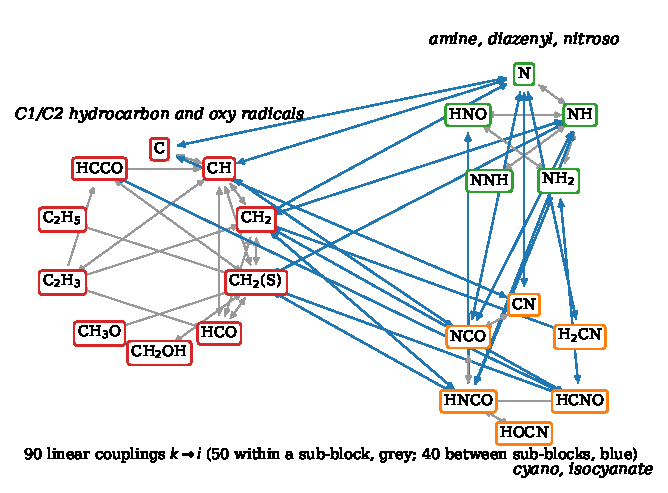
\includegraphics[width=0.95\linewidth]{figs/fig_qss_graph.pdf}
\caption{Linear couplings of the 21 quasi-steady radicals: an arrow $k\to i$ means that a reaction direction with $k$
as its only QSS reactant produces $i$ ($P_{ik}\neq0$ in Eq.~\eqref{eq:qssa}). Grey: within a chemical sub-block; blue: between
sub-blocks. Every radical can reach every other one, so the system cannot be solved one radical at a time.}
\label{fig:qss}
\end{figure}
 A Markowitz order that
eliminates leaf radicals first (\ce{C_{2}H_{5}}, NNH, HOCN, \ce{H_{2}CN}), with common-subexpression elimination, compiles the
solve to 738 floating-point operations, against about 9,300 for a dense $21\times21$ LU (report). The rebuilt
implementation solves the same system by dense LU; the two give the same net production rates of the 22 transported species, with a
maximum relative difference $|\dot\omega_k^{\rm rebuilt}-\dot\omega_k^{\rm original}|/|\dot\omega_k^{\rm original}|$ of
$2\times10^{-8}$ on 400 hot burner states (species whose $|W_k\dot\omega_k|$ exceeds $10^{-3}$ of the largest; checked).

\subsection{Element projection and code generation}
Truncated channels and untransported radicals carry mass, so the reduced system does not conserve elements. The
element deficits are moved into the major products (C into \ce{CO_{2}}, H into \ce{H_{2}O}, N into \ce{N_{2}}, the rest of O
into \ce{O_{2}}). Applied twice, the projection holds C/H/O/N to round-off ($3.96\times10^{-16}$ over full ignition
trajectories, report); without it the drift over a 3\,ms hold reaches $10^{-3}$ relative at $\phi=1$ and
$2\times10^{-2}$ at $\phi=2$ (checked). The compiler emits a dependency-free C++17 header (8.7\,$\mu$s per rate
evaluation\footnote{All computing times in this paper were measured on one machine, sim1: a KVM virtual machine with
16 Intel Core (Haswell) vCPUs, one thread per core, and 62\,GB of memory, running Ubuntu 26.04 and OpenFOAM v2412
(GCC, MPICH). Parallel CFD runs use 8 MPI ranks, i.e.\ 8 processes on 8 cores. The machine was shared with other jobs
(load 12--20 on 16 cores), so absolute times vary by up to about 20\,\% with the load; cost ratios were measured
under similar load. \todo{machine reference or acknowledgement}}) and a vectorized PyTorch version that gives an exact $22\times22$ Jacobian by automatic differentiation.

%% ---------------------------------------------------------------------------------------------------------------
\section{Implementation in OpenFOAM}
\label{sec:impl}

The ARC runs in OpenFOAM v2412 as a chemistry-solver library (arcChemStep), because OpenFOAM's mechanism readers
cannot express quasi-steady species. The case lists only the 22 transported species, with GRI NASA-7 thermodynamics
(lower limit 200\,K), Sutherland viscosity fits and an empty reaction list. For each cell and flow step the library
integrates
\begin{equation}
\frac{dY_k}{dt}=\frac{W_k\,\dot\omega_k(T,\mathbf{c})}{\rho},\qquad
\frac{dT}{dt}=-\frac{\sum_k h_k\,\dot\omega_k}{\rho\,c_p},\qquad k=1,\dots,22,
\end{equation}
at constant pressure over the flow time step, applies the element projection, and returns concentrations at the
starting density, as every OpenFOAM chemistry solver does. The production rates come from the unrolled C++ header; a
table-driven rebuild (26\,$\mu$s per call) agrees with it to $2\times10^{-8}$ in the rates and to $4\times10^{-5}$
in the state after a flow step.

The Jacobian is formed by finite differences (24 right-hand-side calls), so the integrator setting decides the cost.
Table~\ref{tab:integrators} compares OpenFOAM's integrators on 400 hot burner cells over one $2\times10^{-5}$\,s
step, against seulex at relTol $10^{-9}$, absTol $10^{-16}$. Temperature errors are at most 0.01\,K in every row; the
chosen absTol of $10^{-9}$ on $Y$ is still about ten times tighter than the $10^{-10}$\,kmol/m$^3$ of the GA18 and
GRI references. About 90\,\% of the rate calls are Jacobian columns.

\begin{table}[t]
\centering\small
\caption{ODE integrators for the ARC on 400 hot burner cells, one flow step of $2\times10^{-5}$\,s.}
\label{tab:integrators}
\resizebox{\linewidth}{!}{%
\begin{tabular}{lcc}
\toprule
Integrator, relTol / absTol (on $Y$) & Rate calls per cell and step & Max.\ rel.\ error OH / NO / HCN \\
\midrule
seulex $10^{-5}$ / $10^{-12}$ & 873 & $1\times10^{-5}$ / $7\times10^{-6}$ / $2\times10^{-5}$ \\
Rosenbrock34 $10^{-5}$ / $10^{-12}$ & 580 & $1\times10^{-5}$ / $3\times10^{-6}$ / $5\times10^{-6}$ \\
Rosenbrock34 $10^{-4}$ / $10^{-12}$ & 363 & $1\times10^{-4}$ / $8\times10^{-6}$ / $9\times10^{-6}$ \\
\textbf{Rosenbrock34 $10^{-4}$ / $10^{-9}$ (used)} & \textbf{222} & $1.2\times10^{-4}$ / $8\times10^{-6}$ / $6\times10^{-5}$ \\
\bottomrule
\end{tabular}}
\end{table}

Species diffusion uses the constant-Lewis model of the GA18 burner simulation that serves as the starting state and first reference (OF GA18 in Section~\ref{sec:burner}),
$\rho D_k=\lambda/(c_p\,\mathrm{Le}_k)+\mu_t/\mathrm{Sc}_t$ with $\mathrm{Sc}_t=0.7$. The 14 species shared with GA18
keep their Lewis numbers; the 8 new species take theirs from a Cantera counterflow flame with GRI-Mech~3.0 and
mixture-averaged transport, weighted by $|dY_k/dx|$ where $T>600$\,K (\ce{CH_{3}OH} 1.33, \ce{C_{2}H_{2}} 1.34, \ce{C_{2}H_{4}}
1.35, \ce{C_{2}H_{6}} 1.45, NO 1.13, \ce{NO_{2}} 1.22, \ce{N_{2}O} 1.37, HCN 1.30). The OpenFOAM GRI-Mech~3.0 case uses the same
model, with Lewis numbers for all 53 species from the same method.

%% ---------------------------------------------------------------------------------------------------------------
\section{Homogeneous and 1D validation}
\label{sec:val}

Two independent validations against GRI-Mech~3.0 agree: ignition delays are within 0.93\,\% (original) and
1.43\,\% (rebuild), and 1\,atm flame speeds within 1.3\,\% in both. They complement each other in range.

\subsection{Original reduction}
References are Cantera solutions with full \texttt{gri30.yaml}; the ARC is integrated with a BDF method and an exact
enthalpy balance. NO errors use a 5\,ppm floor (Table~\ref{tab:orig}).

\begin{table}[t]
\centering\small
\caption{Validation of the original reduction against GRI-Mech~3.0.}
\label{tab:orig}
\resizebox{\linewidth}{!}{%
\begin{tabular}{lccc}
\toprule
Check & Target & Worst case & Mean \\
\midrule
Transported species & $\le 25$ & 22 (43 skeletal, 53 full) & -- \\
Largest Jacobian eigenvalue, 1800\,K, $\phi=1$ & $\ge100\times$ lower & $3.57\times10^{6}$ vs $4.99\times10^{8}$\,s$^{-1}$ & -- \\
CEMA explosive-mode crossover, 0D / 1D & $\le5$\,\% & 0.51\,\% / 0.00\,\% & -- \\
Element drift, projected & $<10^{-14}$ & $3.96\times10^{-16}$\,kmol/kg & -- \\
Ignition delay, 49 cases (1--10\,atm, $\phi$ 0.6--1.5) & $\le10$\,\% & 0.93\,\% & 0.40\,\% \\
PSR NO, $\tau=3$\,ms, 13 cases & $\le4$\,\% & 1.38\,\% & 0.59\,\% \\
PSR NO, $1.15\,\tau_{\rm bo}$, 13 cases & $\le12$\,\% & 2.99\,\% & 1.63\,\% \\
Laminar flame speed, 15 flames (1 and 5\,atm) & $\le5$\,\% & 4.67\,\% & 1.20\,\% \\
Post-flame NO, 1\,atm flames & $\le4$\,\% & 3.07\,\% & -- \\
\bottomrule
\end{tabular}}
\end{table}

The spectral radius, the largest magnitude among the eigenvalues of the chemical Jacobian, is the inverse of the
fastest chemical timescale and sets the stiffness. At the stoichiometric 1800\,K state, GRI-Mech~3.0 and the skeletal
set share a spectral radius of
$4.99\times10^{8}$\,s$^{-1}$, set by NNH, so pruning alone removes no stiffness; in the ARC the fastest mode belongs to
O, at $3.57\times10^{6}$\,s$^{-1}$. The chain-branching explosive eigenvalue~\cite{lu2010cema} is tracked within
0.17\,\% during induction (1\,atm, 1350\,K, $\phi=1$). PSR NO agrees within 1.4\,\% at $\tau=3$\,ms, where thermal NO
dominates, and within 3\,\% near blow-out, where the prompt, \ce{N_{2}O} and NNH routes dominate: the radicals carried
algebraically (CH, NNH, NCO, HCNO) still feed NO correctly. In a 1\,atm counterflow flamelet, peak $T$ is 2007.1 vs
2012.8\,K and peak NO 165.8 vs 168.8\,ppm. Flame-speed and NO errors grow toward rich mixtures, most at 5\,atm
(Fig.~\ref{fig:1d}).

\begin{figure}[t]
\centering
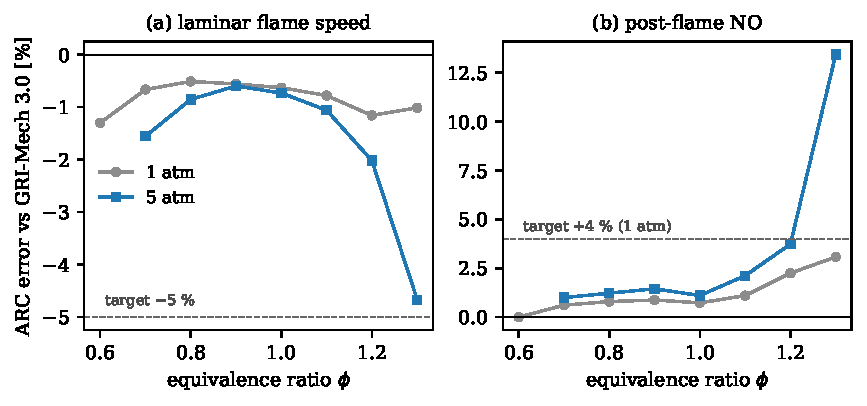
\includegraphics[width=\linewidth]{figs/fig_1d_errors.pdf}
\caption{Error of ARC\_GRI30\_NOx22 against GRI-Mech~3.0 in freely propagating \ce{CH_{4}}/air flames
($T_u=300$\,K): (a) laminar flame speed, (b) post-flame NO (original reduction). The dashed lines are the
acceptance targets fixed before the reduction (Table~\ref{tab:orig}): flame-speed error within $\pm5$\,\% and
post-flame NO error within $\pm4$\,\% at 1\,atm.}
\label{fig:1d}
\end{figure}

\subsection{Independent rebuild}
\label{sec:rebuild}
The mechanism was rebuilt from its specification as a plain-C core (skeletal set, partition, linearized QSSA with the
11 truncated directions, projection). Without the QSSA, the rebuilt rate code reproduces Cantera's net production rates
for gri30\_skel43 to a maximum relative difference of $4\times10^{-9}$ (dimensionless, all 43 species, 30 random
states between 300 and 2400\,K); with the QSSA it matches the original kernel to $2\times10^{-8}$. GRI and the skeletal set run in Cantera
(rtol $10^{-9}$), the ARC in a BDF integrator (rtol $10^{-8}$), in constant-pressure adiabatic reactors of \ce{CH_{4}}
in air; the ignition delay is the time of maximum $dT/dt$ (Table~\ref{tab:ign}). In every case the ARC is closer to
GRI than its skeletal parent: the QSSA partly offsets the skeletal error.

\begin{table}[t]
\centering\small
\caption{Ignition delay, independent rebuild: errors against GRI-Mech~3.0 for $\phi=0.5$\,/\,1.0\,/\,2.0.}
\label{tab:ign}
\resizebox{\linewidth}{!}{%
\begin{tabular}{cccccc}
\toprule
$T_0$ [K] & $p$ [atm] & $\tau_{\rm GRI}$ [ms] & Skeletal-43 [\%] & ARC [\%] \\
\midrule
1200 & 1 & 31.5 / 45.5 / 66.9 & +0.35 / +0.20 / +0.13 & +0.28 / +0.15 / +0.10 \\
1400 & 1 & 2.51 / 3.44 / 4.93 & +0.76 / +0.63 / +0.81 & +0.45 / +0.39 / +0.64 \\
1600 & 1 & 0.401 / 0.468 / 0.596 & +1.04 / +1.25 / +2.12 & +0.32 / +0.51 / +1.43 \\
1100 & 5 & 28.0 / 38.4 / 56.6 & +0.26 / +0.17 / +0.13 & +0.24 / +0.15 / +0.12 \\
1400 & 5 & 0.689 / 0.938 / 1.35 & +0.90 / +0.61 / +0.79 & +0.64 / +0.40 / +0.64 \\
\bottomrule
\end{tabular}}
\end{table}

Three milliseconds after ignition the burnt-gas temperature is within 0.6\,K of GRI for $\phi\le1$ and NO within
1--3\,\%. At $\phi=2$ the ARC is 7--14\,K cooler and its NO 11--16\,\% high, even with the projection applied every
$2\times10^{-5}$\,s; this is the largest error found, in hot rich gas above 2400\,K.

Cantera cannot run a mechanism with quasi-steady species, so the ARC and the skeletal set were run in a purpose-built
1D solver (unsteady premixed flame in the mass coordinate, 1200 nodes, constant-Lewis transport as in the burner), and
the skeletal-to-GRI step was taken from Cantera (Table~\ref{tab:sl}). The combined error is
$(1+\epsilon_{\rm ARC/skel})(1+\epsilon_{\rm skel/GRI})-1$. Constant-Lewis transport alone lowers $S_L$ by 2--3\,\%
relative to mixture-averaged transport, equally for both mechanisms.

\begin{table}[t]
\centering\small
\caption{Laminar flame speed at 1\,atm, $T_u=300$\,K, independent rebuild.}
\label{tab:sl}
\resizebox{\linewidth}{!}{%
\begin{tabular}{ccccccc}
\toprule
$\phi$ & GRI [cm/s] & Skel-43 (Cantera) & Skel-43 (1D) & ARC (1D) & ARC vs skel & ARC vs GRI \\
\midrule
0.7 & 19.51 & 19.36 ($-0.73$\,\%) & 19.06 & 19.09 & +0.12\,\% & $-0.6$\,\% \\
1.0 & 38.05 & 37.87 ($-0.47$\,\%) & 36.91 & 37.01 & +0.29\,\% & $-0.2$\,\% \\
1.3 & 23.69 & 23.50 ($-0.82$\,\%) & 23.03 & $22.91\pm0.10$ & $-0.50$\,\% & $-1.3$\,\% \\
\bottomrule
\end{tabular}}
\end{table}

\subsection{Agreement of the two validations}
Where they overlap the two sets agree: at 1\,atm and $\phi=0.7$, 1.0, 1.3 the original gives $-0.7$, $-0.6$ and
$-1.0$\,\% in $S_L$ and the rebuild $-0.6$, $-0.2$ and $-1.3$\,\%; ignition delays are within 1\,\% in both at
1--5\,atm and $\phi\le1.5$. The rebuild adds $\phi=2$, where the largest error appears; the original adds 10\,atm
ignition, 5\,atm flames (worst: $S_L$ $-4.7$\,\% and NO $+13$\,\% at $\phi=1.3$) and PSR NO near blow-out.

%% ---------------------------------------------------------------------------------------------------------------
\section{Burner flame}
\label{sec:burner}

\subsection{Case and solutions}
The test is a laminar \ce{CH_{4}} jet flame burning under a pot (Fig.~\ref{fig:domain}), on a 2D axisymmetric domain 0.52\,m long and 0.14\,m in
radius (63,087 cells; a 5$^\circ$ wedge in OpenFOAM; gravity along $-x$). A pure \ce{CH_{4}} jet of
$6.735\times10^{-6}$\,kg/s (about 340\,W) issues from $r<2.5$\,mm; an air coflow of $5.77\times10^{-5}$\,kg/s enters
between $r=50$ and 75\,mm, plus 0.05\,m/s outside it; all inlets are at 300\,K. The pot is an unmeshed cylinder at
$x=0.05$--0.20\,m, $r<0.05$\,m, with an adiabatic bottom and convective sides and top
($h=15$\,W/m$^2$K, 323\,K), under a hood with a chimney; the top and the chimney exit are pressure outlets. Radiation
is solved with discrete ordinates, a transparent gas and black walls; the wall-to-wall exchange removes about 45\,\%
of the heat release through the pot bottom, and OpenFOAM reproduces it with its finite-volume discrete ordinates model (fvDOM). The fuel-jet Reynolds number is
about 150. Both codes keep the $k$--$\omega$ SST turbulence model of the original Fluent case active, but the ratio of
its eddy viscosity to the molecular viscosity, $\mu_t/\mu$, stays below 0.06 in the reacting cells, so turbulent
transport is negligible and the flame is effectively laminar.

\begin{figure}[t]
\centering
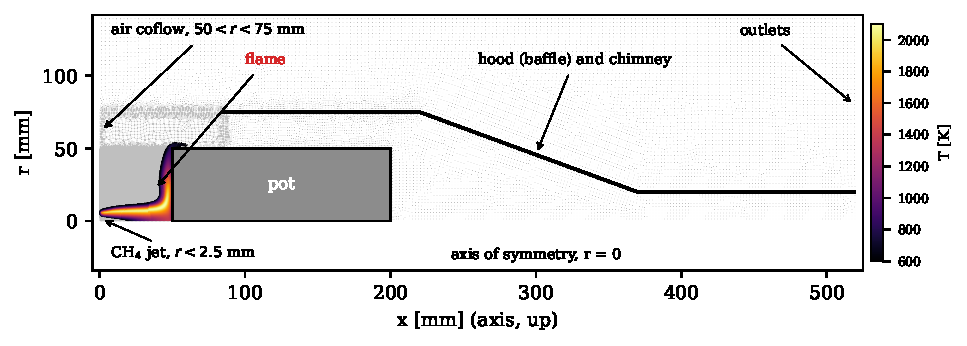
\includegraphics[width=\linewidth]{figs/fig_domain.pdf}
\caption{Burner domain (axisymmetric, axis at the bottom): every cell centre in grey, the flame as the mean
temperature of OF GRI-Mech~3.0 above 600\,K, the unmeshed pot, and the hood baffle leading to the chimney.}
\label{fig:domain}
\end{figure}

Table~\ref{tab:solutions} lists the solutions. OF GRI and OF ARC22 both start from the OF GA18 state at 0.1\,s and run
with $\Delta t=2\times10^{-5}$\,s; snapshots every 2.5\,ms are averaged cell by cell. OF GRI ran to 0.15\,s. OF ARC22
ran to 0.1874\,s. There the temperature of one gas cell on the axis, just below the pot bottom, fell from 300\,K to a
negative value within one time step, which stops the solver. The same cell failed in OF GA18 at 0.1875\,s: the
radiative flux on the axis-adjacent faces of the pot bottom becomes noisy face to face once the fvDOM ray solution
stalls, and the cooling of that cell then runs away. It is independent of the chemistry; the last clean ARC state is
0.185\,s. OpenFOAM cell $i$ is Fluent cell $i+1$
on the identical mesh, so every comparison is cell by cell. Differences are volume-weighted over the full revolution:
the mean hot $|\Delta T|$ uses the cells above 1500\,K in either solution, and the relative L1 of a species is
$\overline{|a-b|}/\overline{\max(a,b)}$ over the cells above 600\,K in either.

\begin{table}[t]
\centering\small
\caption{Burner solutions compared.}
\label{tab:solutions}
\resizebox{\linewidth}{!}{%
\begin{tabular}{llll}
\toprule
Label & Code & Chemistry (direct integration) & Field used \\
\midrule
Fluent GRI & Fluent 20.2 & GRI-Mech 3.0, 53 species & steady \\
Fluent GA18 & Fluent 20.2 & GA18, 18 species & steady \\
OF GA18 (A1r) & OpenFOAM v2412 & GA18, seulex $10^{-10}/10^{-5}$ & mean 0.1--0.1875\,s \\
OF GRI & OpenFOAM v2412 & GRI-Mech 3.0, seulex $10^{-10}/10^{-5}$ & mean 0.125--0.15\,s \\
OF ARC22 & OpenFOAM v2412 & ARC\_GRI30\_NOx22, Rosenbrock34 & mean 0.15--0.185\,s; 0.125--0.15\,s vs OF GRI \\
\bottomrule
\end{tabular}}
\\[2pt]{\footnotesize Fluent: kinetic-theory transport with thermal diffusion. OpenFOAM: constant Lewis numbers,
$\mathrm{Sc}_t=0.7$.}
\end{table}

\subsection{Against Fluent}
Table~\ref{tab:fluent} compares the five solutions. The code difference (48.8\,K with GA18 in both codes) is about
twice the GA18-to-GRI chemistry difference (26.6\,K within Fluent), so a cross-code comparison cannot resolve the
reduction error. Peak NO agrees ($2.48$ vs $2.47\times10^{-4}$), but the NO field differs by 0.37 in relative L1, an
upper bound because NO is still building up in the exhaust at 0.185\,s. Outlet NO$_x$ is not usable: after 87\,ms both
outlets still carry gas from the initial state.

\begin{table}[t]
\centering\small
\caption{Burner flame: the five solutions (top; OF GRI is the mean over 0.125--0.15\,s, the only window it covers) and cell-by-cell differences (bottom).}
\label{tab:fluent}
\resizebox{\linewidth}{!}{%
\begin{tabular}{lccccc}
\toprule
Metric & Fluent GRI & Fluent GA18 & OF GA18 & OF GRI & OF ARC22 \\
\midrule
$T_{\max}$ [K] & 2077 & 2088 & 2121 & 2107 & 2104 \\
$V(T>1500$\,K) [cm$^3$] & 18.08 & 18.25 & 19.94 & 19.46 & 18.79 \\
$V(T>2000$\,K) [cm$^3$] & 2.66 & 2.99 & 3.84 & 3.13 & 3.08 \\
Flame base $x(T>1500$\,K) [mm] & 1.15 & 1.15 & 1.39 & 1.39 & 1.39 \\
OH max [$10^{-3}$] & 3.47 & 3.28 & 3.34 & 3.47 & 3.46 \\
$x$(OH max) [mm] & 16.9 & 15.1 & 15.9 & 19.1 & 17.6 \\
CO max & 0.049 & 0.053 & 0.060 & 0.055 & 0.051 \\
NO / \ce{NO_{2}} max [$10^{-5}$] & 24.7 / 5.5 & -- & -- & 24.0 / 2.8 & 24.8 / 4.0 \\
\ce{N_{2}O} / HCN max [$10^{-5}$] & 0.60 / 11.4 & -- & -- & 0.11 / 10.6 & 0.61 / 14.6 \\
\midrule
Pair & \multicolumn{3}{l}{What differs} & Hot $|\Delta T|$ [K] & OH / CO rel.\ L1 \\
\midrule
Fluent GRI vs Fluent GA18 & \multicolumn{3}{l}{chemistry} & 26.6 & 0.13 / 0.06 \\
OF GA18 vs Fluent GA18 & \multicolumn{3}{l}{code} & 48.8 & 0.22 / 0.12 \\
OF GA18 vs Fluent GRI & \multicolumn{3}{l}{both} & 55.4 & 0.25 / 0.15 \\
OF ARC22 vs Fluent GRI & \multicolumn{3}{l}{code and reduction} & 38.6 & 0.20 / 0.08 \\
OF GRI vs Fluent GRI & \multicolumn{3}{l}{code (GRI chemistry)} & \todo{cloud} & \todo{cloud} \\
OF ARC22 vs OF GRI$^{a}$ & \multicolumn{3}{l}{reduction (same code)} & 3.2 & 0.015 / 0.033 \\
\bottomrule
\end{tabular}}
\\[2pt]{\footnotesize $^{a}$Both averaged over 0.125--0.15\,s (Section~\ref{sec:samecode}).}
\end{table}

\subsection{Same code: ARC against full GRI-Mech 3.0}
\label{sec:samecode}
Both OpenFOAM runs are averaged over 0.125--0.15\,s (11 snapshots each; Table~\ref{tab:samecode},
Fig.~\ref{fig:maps}). Within one code the ARC reproduces the GRI-Mech~3.0 flame to 3.2\,K, so the 38.6\,K against
Fluent GRI is almost entirely code difference. The differences grow slowly with time: over 0.1025--0.125\,s the hot
$|\Delta T|$ was 1.7\,K and the \ce{N_{2}O} L1 0.11. HCN and \ce{N_{2}O}, on the prompt and \ce{N_{2}O}-intermediate routes,
are the weakest species; \ce{N_{2}O} is small in absolute terms (peak $2.6\times10^{-6}$ against $1.1\times10^{-6}$).

\begin{table}[t]
\centering\small
\caption{ARC22 against full GRI-Mech~3.0 in OpenFOAM, mean 0.125--0.15\,s. Totals are domain integrals, ARC/GRI.}
\label{tab:samecode}
\resizebox{\linewidth}{!}{%
\begin{tabular}{lccc}
\toprule
Quantity & OF GRI-Mech 3.0 & OF ARC22 & Difference \\
\midrule
$T_{\max}$ [K] & 2107 & 2108 & +1\,K \\
$V(T>1500$\,K) [cm$^3$] & 19.46 & 19.48 & +0.1\,\% \\
$x$(OH max) [mm] & 19.1 & 19.4 & +0.3\,mm \\
Mean hot $|\Delta T|$ [K] & \multicolumn{2}{c}{--} & 3.2 (max.\ 17) \\
OH / CO / \ce{CO_{2}} rel.\ L1 & \multicolumn{2}{c}{--} & 0.015 / 0.033 / 0.006 \\
NO / \ce{NO_{2}} rel.\ L1 (total) & \multicolumn{2}{c}{--} & 0.071 (1.04) / 0.033 (0.98) \\
HCN / \ce{N_{2}O} rel.\ L1 (total) & \multicolumn{2}{c}{--} & 0.17 (1.21) / 0.23 (1.27) \\
\ce{C_{2}H_{2}} rel.\ L1 & \multicolumn{2}{c}{--} & 0.081 \\
Cost per step, 8 ranks [s] & 30 & 11.2 & $2.7\times$ cheaper \\
\bottomrule
\end{tabular}}
\end{table}

\begin{figure}[t]
\centering
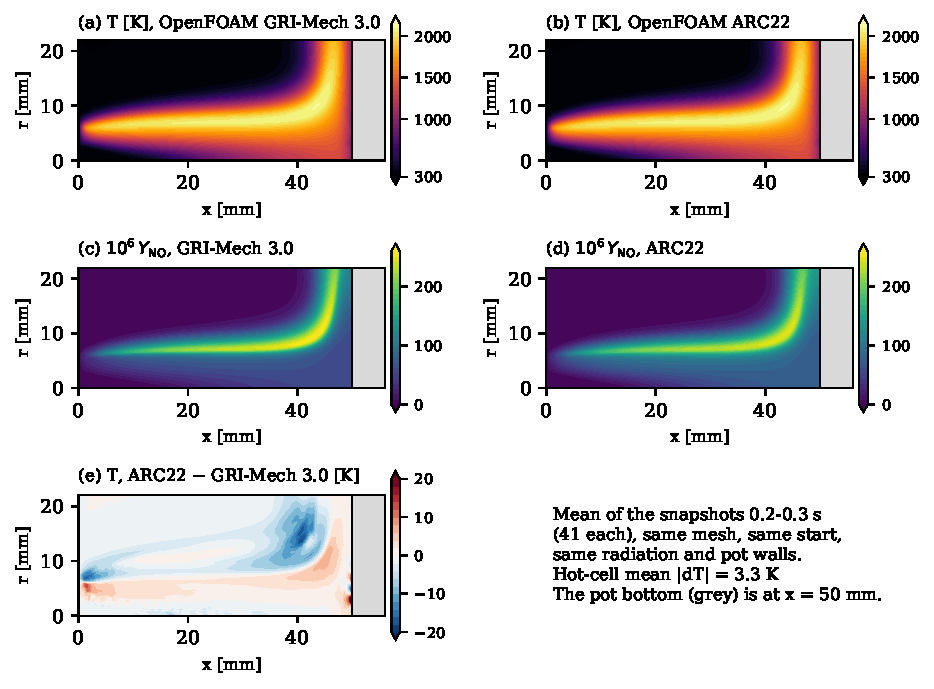
\includegraphics[width=\linewidth]{figs/fig_burner_maps.pdf}
\caption{Mean fields 0.125--0.15\,s below the pot bottom (grey): temperature and NO mass fraction with full
GRI-Mech~3.0 (a, c) and ARC22 (b, d) in OpenFOAM, and their temperature difference (e).}
\label{fig:maps}
\end{figure}

\subsection{Ignition transient}
The ignition test follows the project's fixed CFD evaluation protocol, which freezes the mesh, models, time step
($2\times10^{-5}$\,s), output times and metrics, so that runs that differ only in their chemistry can be compared
snapshot by snapshot. Its ignition phase starts from a uniform lean ($\phi=0.5$) burnt-gas state at 1480\,K: the
fuel jet enters this hot gas at $t=0$ and autoignites. Snapshots are written every 0.5\,ms up to 5\,ms and every
2.5\,ms after; ignition is the first time the domain maximum temperature exceeds 1600\,K. The ARC ran
0--25\,ms and full GRI-Mech~3.0 ran 0--5\,ms in the same code from the same state; OF GA18 (A2r) is a third reference
(Fig.~\ref{fig:ign}). The ARC ignites with GRI-Mech~3.0 (domain $T_{\max}>1600$\,K at 2.8\,ms in both, sampled every
0.2\,ms), and both reach 2060\,K at 5\,ms; GA18 ignites at 2.4\,ms and reaches 2098\,K. The 0.4\,ms earlier ignition of
GA18 is therefore GA18 chemistry, not reduction error. Against GRI, the ARC's mean $|\Delta T|$ over the cells above
600\,K is 0.4--0.6\,K from 1 to 5\,ms; in the burning kernel ($T>1500$\,K) it is 13\,K at 3\,ms and 7\,K at 5\,ms, and
the OH relative L1 is 0.008 throughout. At 3\,ms, while the kernel forms, the ARC kernel is slightly behind
($T_{\max}$ 1871 vs 1896\,K) and early NO and HCN lag (totals 0.75 and 0.80 times GRI); from 4\,ms they run
6--12\,\% high, as in the steady flame. A step costs about 11\,s with the ARC and 37\,s with GRI-Mech~3.0 on 8 ranks.
Up to 25\,ms the ARC flame stays 26.5\,K cooler than GA18, the same GRI-vs-GA18 offset as in the steady flame.

\begin{figure}[t]
\centering
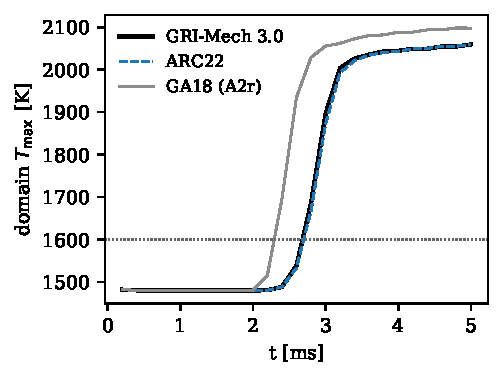
\includegraphics[width=0.6\linewidth]{figs/fig_ignition.pdf}
\caption{Domain maximum temperature during ignition from the lean burnt-gas start, OpenFOAM: full GRI-Mech~3.0,
ARC22 and GA18 (A2r). The dotted line marks the 1600\,K ignition criterion.}
\label{fig:ign}
\end{figure}

%% ---------------------------------------------------------------------------------------------------------------
\section{Discussion and limitations}

\paragraph{What carries the accuracy}
The decoupled nitrogen pass keeps the trace NO$_x$ routes that a single flux-normalized pass would drop, and the
CSP-guided partition puts the fast radicals in the algebraic set, so the QSSA removes the NNH-dominated stiffness that
skeletal pruning leaves in place. The QSSA also partly offsets the skeletal error, so the ARC is closer to GRI than its
43-species parent.

\paragraph{GA18 is not the reference for this flame}
Against OF GA18 in the same code the ARC flame cells ($T>1600$\,K) are 33\,K cooler, with $V(T>1500$\,K)
$\times0.97$, OH L1 13\,\% and CO L1 7\,\%. OF GRI shows the same offset and the ARC tracks it within 3\,K, so the
GA18-based reference flames carry a chemistry bias of about 30\,K against GRI-Mech~3.0.

\paragraph{Weak species and rich gas}
HCN ($+21$\,\% in total) and \ce{N_{2}O} ($+27$\,\%) sit on the prompt and \ce{N_{2}O}-intermediate routes, whose radicals
(CH, NCO, HCNO, NNH) are quasi-steady. The truncated directions include CH\,+\,\ce{CH_{2}}, CH\,+\,HCCO and N\,+\,NCO, a
plausible cause not yet tested; a nonlinear QSSA for that sub-block is the obvious remedy. NO itself stays within
4--9\,\% in total in the flame and during ignition. At $\phi=2$ and $T>2400$\,K the burnt gas is 7--14\,K cool and NO
11--16\,\% high, and rich 5\,atm flames are the worst 1D case; the burner (peak about 2100\,K) does not reach this
regime, but rich high-pressure flames need further checks.

\paragraph{Element projection}
Unprojected drift reaches 2\,\% of the elements at $\phi=2$ over 3\,ms; in a burner, where the gas spends several
tens of milliseconds (0.01--0.1\,s) in the hot region, it would accumulate step after step, so the projection is
required.

\paragraph{Cost}
On 8 ranks a flow step costs 7.6\,s with GA18, 11.2\,s with the ARC and 30\,s with full GRI-Mech~3.0 (37\,s during
ignition): the ARC runs at about 1.5 times the GA18 cost and 2.7--3.4 times faster than GRI. The 140-fold stiffness
reduction does not give a matching speed-up because about 90\,\% of the ARC's rate calls are finite-difference Jacobian
columns; the analytical Jacobian of the PyTorch kernel, ported to the unrolled C++ kernel, is the next speed-up.
Integrator settings matter as much: seulex at $10^{-5}/10^{-12}$ needed four times more rate calls than the setting
used, with no gain in accuracy that matters.

\paragraph{Code-to-code comparison}
Fluent and OpenFOAM differ by 49\,K with identical GA18 chemistry, through species transport (kinetic theory vs
constant Lewis), discretization and radiation details, so a comparison with Fluent GRI-Mech~3.0 validates the ARC only
to that level. The mechanism-specific evidence is the same-code comparison and the NO$_x$ fields that only GRI and the
ARC carry. Cross-code peaks reflect both effects: the ARC $T_{\max}$ is 27\,K above Fluent GRI and its HCN peak
28\,\% higher.

\paragraph{Numerical limits}
The flame windows are short (35\,ms for the ARC mean, 25\,ms for the same-code comparison); $V(T>1500$\,K) still
drifts slowly (19.4 to 18.3\,cm$^3$ over 0.15--0.185\,s) and NO is still building up in the exhaust. All OpenFOAM
flame runs end near 0.187\,s at the same near-axis fvDOM divergence, independent of the chemistry, and outlet NO$_x$
cannot yet be evaluated. Planned remedies, in order: (i) restart from 0.185\,s with the radiation solved at every flow step instead of every
tenth, and more ray-solver iterations; (ii) if the cell still diverges, a finer angular discretization of fvDOM near
the axis or a fixed-temperature condition on the axis corner of the pot bottom; (iii) then extend the ARC and GRI runs
to about 0.3\,s, which gives a common 100\,ms averaging window and lets the burnt gas reach the outlets, so that
outlet NO$_x$ can be compared. \todo{choose and run}

\paragraph{Validation range}
The 0D/1D checks cover ignition at 1--10\,atm and $T_0=1100$--1600\,K up to $\phi=2$, flame speeds at 1 and 5\,atm
($T_u=300$\,K, $\phi=0.6$--1.3), and PSR NO at 1 and 5\,atm. Counterflow extinction and low-temperature
($T_0<1100$\,K) chemistry are not checked.

%% ---------------------------------------------------------------------------------------------------------------
\section{Conclusions}
\begin{enumerate}
\item ARC\_GRI30\_NOx22 transports 22 species, 58\,\% fewer than GRI-Mech~3.0, keeps all six NO$_x$ pathways and is
140 times less stiff.
\item Two independent validations agree: ignition delays within 0.93\,\% (original, 1--10\,atm) and 1.43\,\%
(rebuild, up to $\phi=2$); flame speeds within 1.3\,\% at 1\,atm and 4.7\,\% at 5\,atm in the worst rich case; PSR NO
within 3\,\% down to near blow-out. An independent rebuild from the specification gives the same rates to
$2\times10^{-8}$, so the procedure of Section~\ref{sec:reduction} fully defines the mechanism.
\item As an OpenFOAM chemistry library it runs direct integration of a radiating burner flame at 1.5 times the GA18
cost and 2.7--3.4 times faster than full GRI-Mech~3.0, and adds NO, \ce{NO_{2}}, \ce{N_{2}O} and HCN predictions.
\item In the same code it reproduces the GRI-Mech~3.0 burner flame to 3.2\,K in mean hot-cell temperature, with OH,
CO and NO within 7\,\% (relative L1), and ignites it at the same time (2.8\,ms); HCN and \ce{N_{2}O}, at 17--23\,\%, are
the species to improve.
\item Against Fluent with GRI-Mech~3.0 the gap is 38.6\,K: code-to-code difference (48.8\,K with GA18 in both codes),
not the mechanism. Likewise the earlier ignition and hotter flame of GA18 are GA18 chemistry.
\end{enumerate}

\section*{Data availability}
The mechanism will be provided as Supplementary Material (C++17 header, PyTorch kernel, plain-C core and the
43-species skeletal set in Cantera YAML), together with a short usage note. The generation and validation scripts, the
OpenFOAM chemistry library, the case set-ups, the run scripts, and the per-cell result fields (compressed NumPy files
in Fluent cell order, about 70\,MB) will be archived on Zenodo with a DOI and mirrored in a public GitHub release.
\todo{create the archive and DOI; check that the Fluent case files may be shared}

\section*{Acknowledgements}
\todo{funding and computing resources}

\bibliographystyle{elsarticle-num}
\bibliography{refs}

\end{document}
